% !TEX encoding = UTF-8 Unicode
% !TEX root = ../rapport.tex

\chapter{État de l'art}\label{etat_art}

\section{Modélisation des réseaux de capteurs sans fil}
Dans les différents articles du domaine, les réseaux sans fils sont modélisés sous forme de graphe. Cependant, d'autres paramètres (comme les capteurs) sont modélisés de façon différentes par chaque auteur. Nous allons présenter quelques modélisations possibles pour chaque aspect du problème d'économie d'énergie dans les réseaux de capteurs sans fils.

Tout d'abord, nous allons aborder les paramètres pratiques liés aux réseaux de capteurs. Nous formaliserons ensuite la modélisation d'un réseau par les graphes. Puis nous aborderons les différents modèles énergétiques. Enfin, nous nous pencherons sur les définitions de durée de vie d'un réseau. Une table récapitulative des notations est disponible à la fin de cette partie.

\subsection{Critères pratiques}\label{modelePratique}


Différents modèles sont possibles :

% TODO : citer les articles qui utilisent telle ou telle modélisation
La modélisation de base des réseaux de capteurs sans fil \textbf{$M_1$}:

\begin{itemize}
 \item \textit{Uniformité.} Tout les capteurs sont identiques (batterie, portée, capacité de calcul…).
 \item \textit{Connexité.} Le réseau est initialement connexe (chaque capteur est lié directement ou indirectement à tous les autres).
 \item \textit{Planarité.} Les capteurs sont place dans un plan euclidien à deux dimensions (distance euclidienne).
 \item \textit{Staticité.} Pas de mobilité des capteurs : nous supposerons que les capteurs sont immobiles.
 \item \textit{Sans ajout de capteurs.} Le réseau comprend un nombre fixe de capteurs $n$. Aucun ajout de capteurs en cours de fonctionnement n'est possible.
 \item \textit{Transmission idéale.} Dans des conditions de transmission de message idéales : aucune interférence entre les messages, pas de perturbations des ondes, système d'identifiants uniques.
 \item \textit{Fiabilité.} Les capteurs sont fiables, aucune panne n'est possible.
 \item \textit{Energie initiale fixée.} Chaque capteur a une énergie initiale $\beta$ donnée. Un modèle décrit la consommation énergétique. Un capteur est éliminé lorsqu'il n'a plus d'énergie ou que son énergie 
 restante ne permet plus aucun envoi de message. 
 \item \textit{Egalité.} Chaque site peut à tout moment débuter une procédure de transmission de données. Une loi de probabilité modélise ce phénomène (loi de poisson).
 \item \textit{GPS.} Chaque site connait sa position absolue.  \\
\end{itemize}

D'autres modèles plus complexes mais plus réalistes prennent en compte:
  
\begin{itemize}
   
 \item L'ajout de capteurs: le réseau comprend un nombre variable de capteurs $n$. Les ajouts de capteurs en cours de fonctionnement sont possibles.
 \item Les capteurs peuvent tomber en panne en raison de divers facteurs. Une loi de probabilité modélise ce phénomène.   
 \item La mobilité des capteurs. La position de chaque capteur varie au cours du temps.
 \item Les capteurs ne sont pas forcément identiques (batterie, portée, capacité de calcul, connaissance du réseau...).
 \item Espace en 3 dimensions.
 \item Interférences radio.
 \item Modèle de consommation énergetique complexe.
 \item ...
\end{itemize}


\subsection{Modèle d'un réseau de capteurs : un graphe}

 \paragraph*{} Un WSN peut être représenté par un graphe $G= (V,E,\gamma)$ où :
 \begin{itemize}
 \item $V$ est un ensemble de noeuds (capteurs)
 \item $E \subseteq V \textsuperscript{2}$ est l'ensemble des arêtes représentant les communications possibles entre les capteurs: $(u,v)$ appartient à $E$ signifie que $u$ peut envoyer un  message à $v$
 \item $\gamma$ est le rayon d'émission maximum
 \end{itemize}
 
 On note $ n=|V| $ la taille du WSN. Notons que les éléments de E dépendent de la
 position des capteurs ainsi que de leur portée. Nous supposerons que tout les capteurs ont la même portée maximale notée $\gamma$. 

%%%%%%%%%%%%%%%%%%%%%%%%%%%%%%%%%%  Distance

\begin{mydef}
Nous noterons $ij$ l'arête allant de $i$ à $j$. \\
Nous noterons $d_e(u,v)$ la \textit{distance euclidienne} dans $\mathbb{R} \textsuperscript{2}$ entre $u$ et $v$:
$$E = \{ (u,v) \in V ^{2} \mid d(u,v) \leq \gamma \}$$
Nous noterons $d_G(u,v)$ la \textit{distance} entre $ u $ et $ v $ : $d_G(u,v)= \min\limits_{k \in \mathbb{N}}(k \mid v \in N_k(u))$
\end{mydef}


%%%%%%%%%%%%%%%%%%%%%%%%%%%%%%%%%%   Graphe unité
\begin{mydef}
 On appelera $G= (V,E,\gamma)$ le \textit{graphe unité} du WSN et $\gamma$ son rayon de communication.
\end{mydef}



%%%%%%%%%%%%%%%%%%%%%%%%%%%%%%%%%%   Voisinage
\begin{mydef}
Nous noterons le 1-voisinage de $u$ : $N_1(u) = \{ v \in V  \mid (u,v) \in E \}$ \\
Nous noterons le 2-voisinage de $u$ : $N_2(u) = \{ v \in V \mid  \exists w \in V :\{(u,w);(w,v)\} \in E ^2\}$ \\
Nous noterons le $k$-voisinage de $u$, $k \in \mathbb{N} : N_k(u) = \{ v \in V  \mid \exists $ un chemin $c (u,v): |c| \leq k\}$.\\
Nous parlerons de 1- 2- et k-voisins de $i$ pour désigner des noeuds appartenant respectivement
 à $N_1(i), N_2(i),N_k(i)$. \\
Soit $A \subseteq V$, on note $N(A) = \{ v \in V\textbackslash  A \mid \forall u\in A,(u,v) \in E \}$ \\
Le degré de $ u $ est le nombre  $N(u)=|N_1(u)|$.\\
\end{mydef}

%%%%%%%%%%%%%%%%%%%%%%%%%%%%%%%%%%   Diametre
\begin{mydef}
Nous noterons $diametre_G= \max\limits_{i,j\in \textlbrackdbl 1,n \textrbrackdbl,i<j} (d_G(i,j))$.
\end{mydef}
 

\begin{figure}[H]
\centering
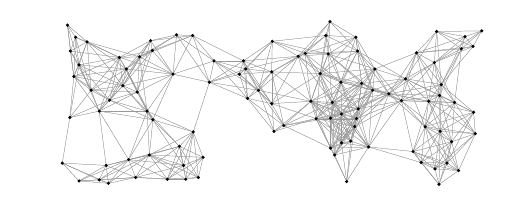
\includegraphics[scale=0.5]{Etat_de_l'art/source/graph1.png}
\caption{Graphe unité}
\end{figure} 



%%%%%%%%%%%%%%%%%%%%%%%%%%%%%%%%%  Densité, distance moyenne
\begin{mydef}
 
 Le degré de $G$ est la moyenne des degrés de chaque sommet : $$N_G=\sum_{i=1}^n{\frac1n N(i)}$$\\
 La densité de $G$ est le nombre $D_G=N_G/diametre_G$\\
 La distance de $G$ est la moyenne des distances entre toutes paires de sommets:$$d_G=\sum_{i,j\in \textlbrackdbl 1,n \textrbrackdbl,i<j}{\frac1n d_G(i,j)}$$
 La distance euclidienne de $G$ est la moyenne des distances euclidienne entre toutes paires de sommets:$$d_e(G)=\sum_{i,j\in \textlbrackdbl 1,n \textrbrackdbl,i<j}{\frac1n d_e1(i,j)}$$

\end{mydef}


\subsection{Modèle énergétique}
\subsubsection{Energie d'un capteur}
Dans \cite{Dong2005}, Dong présente les deux modèles de consommation énergétique communément utilisés.
\paragraph{The Packet based model.}
Nous utiliserons pour notre analyse le modèle de consommation d'énergie idéal suivant:
nous considèrerons que chaque capteur $i$ a une énergie initiale $E_{init}=\beta$.
L'envoi de message est le seul facteur de perte d'énergie. L'énergie consommée lors de la réception de message, l'acquisition et traitement des informations sera considérée comme négligeable.
Tous les capteurs $i$ offrant les mêmes caractéristiques, ils peuvent modifier leur rayon d'émission $r_i$ en respectant l'inégalité suivante : $0 \leq r_i \leq \gamma$.
Nous noterons $E_i$ l'énergie restante de $i$.
L'envoi d'un message de $i$ avec un rayon $r$ coûte $$ E(r)= \begin{cases} r^\alpha + c & \text{si }i\neq j \\ 0 & \text{sinon}  \end{cases}$$
L'envoi d'un message de $i$ à $j$ ($d_e(i,j)\leq \gamma$) coûte  $ E_{ij}=E(d_e(i,j))$.

\paragraph{The Time based model.}
Ce modèle plus réaliste prend en compte l'énergie de réception des messages, de traitement ainsi que d'écoute inactive du réseau (mode veille).
En effet, dans \cite{Kasten2001}, Kasten souligne le fait que souvent, la réception, l'écoute et le traitement consomment en moyenne autant d'énergie que la transmission de message.
Dans de nombreuses topologies, si la fréquence des transmissions est faible, beaucoup de capteurs vont être à court d'énergie avant même d'avoir pu transmettre des messages.
Dans beaucoup d'applications, la densité du réseau étant élevée, le coût propre aux transmissions de message est relativement faible tandis que le coût de réception des messages est élevé puisque chaque capteur traite les messages de son voisinage (qui en l'occurence est grand).



\paragraph{Energie globale.}
\begin{mydef}
 L'énergie potentielle de G est la somme des énergies des capteurs :$$E_G=\sum_{i=1}^n{E_i}$$
 La consommation de  G est :$$C_G=n\beta - E_G$$
 Le coût moyen de transmition de  G est :$$c_G=E(d_e(G))$$
 Le cout moyen d'un broadcast est $C(1)$.\\
 Le cout moyen de $k$ broadcast est $C(k)$
\end{mydef}
% TODO : singlecast


\subsection{Durée de vie du réseau}
\subsubsection{Problématique}


Dans un réseau de capteurs sans fil, la contrainte majeure est l'efficacité de l'algorithme utilisé en matière de consommation énergétique. En effet, la principale caractéristique des capteurs
est leur petite taille et leur micro-batterie. Dans la majeure partie des cas, remplacer les batteries est impossible. Cependant la durée de vie d'un WSN est difficile à définir et à mesurer.
Il n'y a pas de définition absolue. Elle indique combien de temps le réseau sera 'efficace' par rapport à l'application donnée (nombre de transmissions effectuées, connexité du réseau, pourcentage de noeuds vivants...).

% TODO : citer les articles correspondants aux deux approches ci-dessous
Dans la littérature, deux approches apparaissent clairement en matière de maximisation de la durée de vie des WSNs. Une approche indirecte consiste à minimiser la consommation d'énergie de façon locale tandis que l'autre a pour but 
de maximiser la directement la durée de vie du réseau de façon plus globale. Bien que l'approche indirecte puisse améliorer la durée de vie du réseau, elle ne suffit pas à elle seule à appréhender le problème de la durée de vie.
Parmi ces approches figurent  par exemple le fait de maximiser le nombre de transmissions effectuées avant qu'un capteur ne meurt.

Dans \cite{Liang2002}, Liang prouve que le  problème THE MINIMUM-ENERGY BROADCAST
TREE PROBLEM est NP-complet par réduction à (3-CNF SAT):
\begin{myth}
Soient un WSN $G$ dans lequel chaque noeud a $k$ rayons de transmission possibles, une source $s$ et un entier positif $w$.
Déterminer s'il existe un arbre de broadcast de source $s$ tel que la somme des coûts de transmission aux noeuds relais (qui ne sont pas des feuilles) soit inférieure à $w$ est NP-Complet.
\end{myth}
Ainsi, pour un broadcast donné il n'existe pas d'algorithme centralisé polynomial pour trouver l'arbre de diffusion optimale. Il est évident qu'il n'en existe pas de distribués. 
Dans \cite{Dong2005}, Dong prouve que le  problème BROADCAST LIFETIME est NP-Complet par réduction de (3DM):
\begin{myth}
Soient un WSN $G$, une source $s$ et un entier positif $k$.
Déterminer si G a assez d'énergie pour broadcaster $k$ messages a partir de $s$ est NP-Complet.
\end{myth}

De façon formelle, il est donc souvent impossible de calculer le nombre total de broadcasts réussis étant donné un réseau et un protocole (sauf quand le protocole est très simple $cf$ \ref{algosSansBalisage}). Nous analyserons 
donc \textit{les performances moyennes} des algorithmes quand cela est possible. Sinon, les simulations nous permettrons de mesurer les performances en fonction de différentes topologies.

\subsubsection{Définitions}
Les définitions et critères de durée de vie d'un WSN sont tirés des articles \cite{Dietrich2009},\cite{Champ2009lifetime},\cite{Elleithy2011}. 

\begin{mylt}
Nombre moyen de transmissions réussies avant qu'un capteur n'ai plus de batterie (TTFF).
\end{mylt}
\begin{mylt}
Nombre moyen de transmissions réussies avant que le réseau ne perde sa connectivité.
\end{mylt}
\begin{mylt}
Nombre moyen de transmissions réussies jusqu'à ce qu'il ne reste que $X\%$ de noeuds vivants.
\end{mylt}


\subsection{Rayon optimal d'émission}
% TODO : relecture Rayon optimal d'émission et ajout à l'intro de la section
\begin{myth}
Sans chevauchement et sans vide, un plan ne peut être découpé de façon uniforme que par des polygones réguliers de type triangle, carrés ou hexagones.
\end{myth}
\begin{proof}
Soit $m$ le nombre de sommets d'un $m$-polygone et $n$ le nombre de $m$-polygones nécessaires pour couvrir $2\pi$ degrés. Nous avons: 
$$\frac{(m-2)n\pi}{m}=2\pi$$
$$\Leftrightarrow$$
$$(m-2)(n-2)=4$$
Comme $n$ et $m$ sont des entiers, les seules solutions sont : 
$$(m-2;n-2)\in\{(1,4),(2,2),(4,1) \}$$
$$\Leftrightarrow$$
$$m \in \{ 3,4,6 \}$$
\end{proof}

\begin{myth}
Le quadrillage en hexagone est celui offrant le moins de chevauchements du point de vu WSN. Nous admettrons ce théorème.
\end{myth}
%\begin{figure}[H]
%\centering
%\includegraphics[scale=0.7]{Etat_de_l'art/source/hexagone1.png}
%\caption{ Chevauchement d'un maillage hexagonale}
%\end{figure} 

Soit $P$ un plan sur lequel $n$ capteurs sont placés. Chaque capteur peut émettre des messages avec un rayon compris entre 0 et $\gamma$. Dans ce protocole, tout les nœuds auront un même rayon d'émission fixe $R$.
Etant donnée une source $s$ et un message $M$ à broadcaster, nous devons placer les noeuds relais de façon a minimiser leur nombre $m$. Bien sûr, leur nombre dépend directement du rayon $R$.
 

Dans un réseau hexagonal, nous avons les résultats suivants :
Soit $S$ l'aire du plan rectangulaire $P$. Connaissant $R$, nous pouvons calculer facilement le nombre de sommet pour couvrir le plan.
Soit $h$ le nombre d'hexagones couvrant $P$: 
Knowing r is the exact distance between two emitting
nodes, we can easily compute the necessary quantity of them
to cover the entire area. To do this, we just have to find how
many hexagons, denoted by h, fit on our area of surface S:
$$h \simeq \frac{Surface ( P)}{Surface(hexagone)}=\frac{2S}{3R^2 \sqrt{3}}$$

Comme il faut deux noeuds par hexagone,$$n=2h=\frac{4S}{3R^2 \sqrt{3}}= \frac{k}{R^2}$$ où $k=\frac{4S}{3 \sqrt{3}}$

Ainsi, le cout d'un broadcast vaut: $$C(1)(R)= n\cdot E(R)=\frac{k}{R^2}\cdot E(R)=\frac{k}{R^2}\cdot (R^\alpha+c)$$
Nous cherchons le rayon optimal minimisant $C(1)(R)$. Comme $\alpha\geq 2$, $c\geq 0$ et $R>0$, nous avons 4 cas possibles:
\begin{itemize}
 \item $\alpha=2$, $c=0$: nous avons $C(1)(R)=k$. $R_{opt}$ ne depend pas de $r$.
 \item $\alpha=2$, $c\neq0$: nous avons $C(1)(R)=k(1+cR^{-2})$. Au plus le rayon doit etre le plus gran possible: $R_{opt}=\gamma$
 \item $\alpha>2$, $c=0$: nous avons $C(1)(R)=kR^{\alpha-2}$. $R_{opt}=0$
 \item $\alpha>2$, $c\neq 0$: nous avons $C(1)(R)=k(R^{\alpha-2} + c R^{-2} ) $.\\
 En derivant, nous obtenons: $C'(1)(R)= k( (\alpha 2) R^{\alpha-3}- 2cR^{-3} ) $.\\
D'ou: $$R_{opt}=\sqrt[\alpha]{\frac{2c}{\alpha-2}}$$
\end{itemize}

Biensur, en pratique, il est impossible sur un topologie quelquonces d'extraire un tel maillage hexagonale. Cependant, l'idée des algorithmes de broadcast est de choisir les noeuds relais de façon à ce que leur ensemnble se rapproche 
au maximum d'un tel maillage.



\begin{table}[H]
{%
\newcommand{\mc}[3]{\multicolumn{#1}{#2}{#3}}
\begin{center}
\begin{tabular}{|c|l}
\hline
$G(V,E,\gamma)$ & \mc{1}{c|}{Graphe unité}\\\hline
$n$ & \mc{1}{c|}{Nombre de capteurs}\\\hline
$\gamma$ & \mc{1}{c|}{Rayon d'émission maximum}\\\hline
$\alpha$ & \mc{1}{c|}{Constante de consommation énergetique}\\\hline
$c$ & \mc{1}{c|}{Constante de consommation énergetique}\\\hline
$\beta$ & \mc{1}{c|}{Energie initiale des capteurs}\\\hline
$E_i$ & \mc{1}{c|}{Energie restante de $i$}\\\hline
$E_{ij}$ & \mc{1}{c|}{Coût d'envoi d'un message de $i$ à $j$}\\\hline
$N(u) $& \mc{1}{c|}{Degré de u}\\\hline
$d_G(i,j)$ & \mc{1}{c|}{Distance dans G entre $i$ et $j$}\\\hline
$d_e(i,j)$ & \mc{1}{c|}{Distance euclidienne entre $i$ et $j$}\\\hline
$N_k(u)$ & \mc{1}{c|}{Nombre de k-voisins de u }\\\hline
$N_G$ & \mc{1}{c|}{Degré de G}\\\hline
$d_G$ & \mc{1}{c|}{Distance de G}\\\hline
$d_e(G)$ & \mc{1}{c|}{Distance euclidienne de G}\\\hline
$diametre_G$ & \mc{1}{c|}{Diametre de G}\\\hline
$D_G$ & \mc{1}{c|}{Densité de G}\\\hline
$C(k)$ & \mc{1}{c|}{Coût de $k$ broadcasts}\\\hline

\end{tabular}
\end{center}
}%
\caption{Notations}
\end{table}



\section{Algorithmes existants}\label{class}

Les réseaux de capteurs sans fils constituent un domaine de recherche récent et actif. Une grande quantité d'articles ont été publiés cette dernière décénnie. Nous n'en aborderons que quelques uns.


\subsection{Eléments de classification}
Les éléments de classification cités ci-dessous sont inspirés des articles \cite{stojmenovic2004}, \cite{ingelrest2005}, \cite{wu2003}.



\subsubsection{Transmissions en broadcast vs transmissions en single-cast}
Dans un réseau $G(V,E,\gamma)$, deux capteurs peuvent communiquer directement uniquement s'ils sont 1-voisins dans G. A cause l'atténuation du signal wifi, le rayon de transmission est relativement limité, c'est pourquoi les communications doivent se faire par multi-sauts. Tout ceci est géré par un algorithme de routage. Les algorithmes de routage peuvent gérer le broadcast (un nœud vers tous les autres) et/ou le single-cast (un nœud vers un autre). Chacune des approches a des avantages dans un contexte précis.

% TODO : citer des articles
La procédure de broadcast est un mécanisme fondamental pour la propagation des données ainsi que pour la découverte de routes. En effet le broadcast est utilisé pour acquérir une connaissance du voisinage des capteurs. L'avantage de ce mode de transmission est qu'avec une seule émission, tout le voisinage est averti. Le routage des broadcasts nécessite de s'assurer que le message ne soit pas indéfiniment retransmis mais que tous les nœuds du graphe soient touchés. Parfois même si le destinataire est à distance 1 dans le graphe unité, il est nécessaire que le message soit relayé par un nœud tiers pour des raisons énergétiques.

% TODO : single-cast / multi-cast

\subsubsection{Algorithme à rayon d'émission fixe vs variable}
% TODO


\subsubsection{Algorithme global vs local}
Le fait qu'un algorithme soit global ou local dépend du type d'informations qu'il utilise. Si un capteur connait dès son arrivée des informations sur ses voisins, l'algorithme est global. À l'inverse, un algorithme distribué fournit aux capteurs uniquement les informations que leurs perceptions peuvent leur procurer.

Cependant, la distinction entre global et local n'est pas toujours évidente. Des algorithmes centralisés peuvent être implémentés d'une manière distribuée en décidant par exemple d'un noeud possédant la connaissance globale du réseau. À l'inverse, un algorithme distribué peut simuler une connaissance globale : au travers d'un échange séquentiel et très localisé d'informations  (1 ou 2-voisinage par exemple), chaque noeud peut combiner sa connaissance avec celle de ses voisins et ainsi obtenir une vision globale du réseau. Cependant, une telle phase de propagation coûte très cher en terme de nombre de messages échangés et de temps.

Si le réseau est dynamique (mobilité des capteurs), maintenir une connaissance locale du réseau devient plus complexe tandis que tenir à jour la topologie globale de celui-ci devient impossible par le moyen cité précédemment. Ainsi, la quantité et la nature des informations nécessaires au déroulement de l'algorithme sont une bonne mesure de la capacité d'adaptation du protocole à un environnement dynamique.   

Les algorithmes peuvent entrer dans une des catégories suivantes :
\begin{description}
 \item[Global :]protocole de routage, centralisé ou distribué nécessitant une connaissance globale du réseau.
 \item[Quasi-global :]protocole distribué de broadcast nécessitant une connaissance quasi-globale du réseau.
 \item[Quasi-local :]protocole distribué nécessitant une connaissance du réseau principalement locale et occasionnellement globale (ex: Cluster networks: tandis que les groupes peuvent être construits de manière locale, des réactions en chaines peuvent arriver).
 \item[Local :]protocole distribué nécessitant une connaissance très locale du réseau. Tous les algorithmes de 1 ou 2-voisinage appartiennent à cette catégorie.
\end{description}

Remarquons que pour qu'un protocole soit extensible, il doit être avant tout distribué et local :  le comportement de chaque noeud, bien qu'il nécessite qu'une connaissance locale du réseau, permet d'atteindre l'objectif global. Il est facile d'admettre que l'extensibilité d'un WSN est inversement proportionnelle à la localité du protocole.



\subsubsection{Algorithme à balisage vs algorithme sans balisage (beaconless)}
Les algorithmes 'beaconless' ne nécessitent pas de phase d'initialisation ni de mise à jour. Les nouveaux capteurs sont immédiatement opérationnels mais n'ont aucune connaissance de leur environnement et notamment de leur voisinage dans G. 

Dans les algorithmes avec balisage, tout capteur, lorsqu'il est connecté au réseau, commence par une procédure d'initialisation et stocke en mémoire un certain nombre d'informations (voisins, groupe, topologie locale...). Au cœur de l'algorithme, chaque noeud met périodiquement à jour ces informations. Il est possible, par exemple, que chaque site envoie régulièrement à ses voisins un message de type
'Hello' contenant par exemple son Id, sa position, sa dominante connexe, son degré, ses voisins, etc.



\subsubsection{Algorithme déterministe vs probabiliste}
Un protocole de broadcast peut utiliser des fonctions probabilistes pour prendre certaines décisions de manière aléatoire.
% TODO : déterministe, développement de probabiliste



\subsection{Quelques algorithmes de routage}
% TODO : harmoniser les durées de vie ou poser les notations dans l'intro de la subsection
% TODO : citation de tous les articles (ou références)

%\subsection{Algorithmes sans balisage}\label{algosSansBalisage}


\subsubsection{Blind Flooding}
Le "blind flooding" ou "broadcast aveugle" est un algorithme glouton de broadcast sans balisage. Lors de la réception d'un message par un noeud, si c'est la première fois qu'il le reçoit, il le broadcast à ses voisins (avec le rayon maximum), sinon il ne fait rien.

\emph{Consommation} :  le coût global d'un broadcast est exactement le coût moyen puisque chaque noeud $i$ envoie un unique message <$M$,$\gamma$> par broadcast.
Le coût global d'un broadcast est $C(1) = n \cdot E( \gamma )= n\cdot \gamma^\alpha +  n\cdot c $.
Le coût global de $k$ broadcasts est $C(k) = k\cdot n \cdot E( \gamma )= k\cdot n \cdot \gamma^\alpha +  k \cdot n\cdot c $.

\emph{Durée de vie} :   $$LT(Blind Flooding)=\lfloor \frac{\beta}{n\cdot \gamma^\alpha +  n\cdot c} \rceil$$



\subsubsection{Probabilistic Flooding}
Afin d'éviter le redondance et les collisions, une idée est que chaque noeud retransmette le message suivant une probabilité $P$ lorsqu'il le reçoit pour la première fois. Si $P=1$ cela équivaut au blind flooding.

\emph{Consommation :} Chaque noeud ayant un probabilité $P$ de retransmettre le message <$M$,$\gamma$>, en moyenne $P\cdot n$ nœuds envoient ce message lors d'un broadcast.
Le coût moyen d'un broadcast est $C(1) = P\cdot n \cdot E( \gamma ) $. Le coût global de $k$ broadcasts est $C(k) = P\cdot k\cdot n \cdot E( \gamma ) $ .

\emph{Durée de vie :} $$TTFF(Probabilistic Flooding)=\lfloor \frac{\beta}{P \cdot (n\cdot \gamma^\alpha +  n\cdot c)} \rceil$$


% TODO : reprendre la relecture depuis ici
\subsubsection{Area-based Beaconless Broadcasting Algorithms \cite{Ovalle2006}}
Nous supposons que les noeuds n'ont aucune connaissance de leur voisinage. Cependant ceux-ci connaissent leur position géographique (GPS par exemple). Chaque capteur a un rayon d'émission fixe $R$ et couvre une zone circulaire.
%\begin{figure}[H]
%\centering
%\includegraphics{Etat_de_l'art/source/abba.png}
%\caption{ }
%\end{figure} 

L'idée maitresse de ABBA est assez simple. A la première réception d'un message, le nœud initialise un timer. Avant expiration du timer, le noeud peut recevoir d'autres copies du même message. Si un nœud $u$ reçoit le même message de différentes sources et que ces sources couvrent sa zone, cela signifie que chacun de ses voisins potentiels a déjà reçu le message. Alors $u$ ne retransmet pas le message et quand que son timer expire, il ne fait rien. Sinon si le voisinage de $u$ n'est pas couvert alors $u$ retransmet.

Comme chaque couverture est un cercle de rayon $R$, le critère de couverture peut être simplifié : au lieu de s'intéresser au disque entier, un noeud vérifie uniquement si le périmètre $\pi$ de sa zone est couvert par ses voisins lui ayant envoyé le message.


\begin{algorithm}[h]
\caption{ABBA}
\label{ABBA}
\begin{algorithmic}
\REQUIRE:
Un noeud source $s$, un message $M$
\STATE $s$ envoie  <$M$,$s$,$position_s$,$R$> ;
\STATE Réception  par  $u$ de  <$M$,$v$,$position_v$,$R$>
\STATE $z_u\leftarrow ensemble_{vide}$ ;
\STATE Calculer la zone $z$ couverte par $v$ lors de la transmission;
\STATE Déclencher le timer;
\REPEAT
    \STATE Attendre la réception d'un autre copie de $M$ ou que le timer expire;
    \IF {Une copie de $M$ est reçue}
	\STATE Mettre à jour $z_u$;
	\STATE réinitialiser le timer;
    \ENDIF
\UNTIL{timer expire;}
\IF {$\pi \nsubseteq z_u$}
    \STATE Retransmettre;
\ENDIF
     \STATE Ignorer les autres copies de M;

\end{algorithmic}
\end{algorithm}


%\subsection{Algorithmes globaux}


\subsubsection{Broadcast Incremental Power protocol \cite{Wieselthier2000}}

  Rappelons les désavantages des transmissions longue portée: interférences, cout énergétique (le modèle de consommation énergétique des noeuds est non linéaire par rapport au rayon à cause de l'atténuation du signal radio).
C'est pourquoi il est nécessaire de trouver le bon compromis entre le rayon de transmission et le nombre de messages circulant : un large rayon de transmission coute cher mais atteint beaucoup de nœuds ; un court rayon cout très peu cher mais augmente le nombre de messages. 

'Boadcast Incremental Protocol' est glouton et centralisé. Il se base sur l'algorithme de Prim \cite{Prim1957} : un algorithme permettant de construire un arbre couvrant de poids minimum à partir d'un sommet d'un graphe. Le principe de l'algorithme de Prim est de construire l'arbre couvrant minimal arête par arête. Pour ajouter une arête à un arbre partiellement construit, il considère l'ensemble des arêtes dont une extrémité est connectée à l'arbre déjà construit, et l'autre extrémité ne l'est pas. Il choisit dans cet ensemble une arête de poids minimal qu'il ajoute à l'arbre. L'algorithme commence avec un arbre couvrant contenant un nœud et pas d'arêtes, et ajoute successivement $n-1$ arêtes.

La formation d'un arbre couvrant de poids minimum dans BIP suit le même principe dans le sens où les arêtes sont une par une ajoutées à l'arbre. En fait, BIP utilise l'algorithme de Prim avec une différence fondamentale : au lieu d'utiliser des coûts fixes $P_{ij}$ sur les arêtes (demeurant inchangés au cours de la procédure), BIP actualise dynamiquement ces couts $P'_{ij}$ à chaque étape ($i.e$ à chaque ajout d'une arête) ; ce qui traduit le fait que le coût d'ajout d'une arête dépends des noeuds déjà dans l'arbre de la façon suivante : 
$$ \forall i \in BIP, \forall j \notin BIP, P'_{ij}=P_{ij}-P(i)$$
où $P_{ij}$ est le coût réel de transmission et $P(i)$ le coût de broadcast de $i$ dans l'arbre.
$$\begin{cases}
	P(i)=0\ si\ i\ est\ une\ feuille\\
	P(i)=\max\limits_{j\in N_1(i)\bigcap BIP}(E_{ij})\ sinon\\
\end{cases}$$
 $P'_{ij}$ représente donc le coût d'ajout de $j$ par un noeud $i$ appartenant au sous ensemble des feuilles
directes de $i$(ou $i$ lui meme si c'est une feuille). La paire $\{i,j\}$ minimisant $P'_{ij}$ est selectionnée et $i$ transmet à $j$. Ainsi, une nouveau arete est ajoutée a chaque etape de l'algorithme.\\



\begin{algorithm}[h]
\caption{Procédure de construction du BIP-Tree}
\label{algo_BIP_tree}
\begin{algorithmic}
\STATE ENTREES  $G=(V,E)$ un graphe connexe, $s$ une source, un cout de transmition $P_{ij}$
\STATE SORTIE  Arbre BIP de racine s
\STATE B : ENSEMBLE des arêtes de l'arbre
\STATE  $B \leftarrow arbre_{vide}$
\STATE Marquer $s$
\STATE Creer les nouveaux poids: $\forall j \notin BIP, P'_{sj}=P_{sj}-P(s)=P_{sj}$
\WHILE {il existe un sommet non marqué adjacent à un sommet marqué }
   \STATE Mettre à jour les poids:  $ \forall i \in BIP, \forall j \notin BIP, P'_{ij}=P'_{ij}-P(i)$
   \STATE Sélectionner un sommet j non marqué adjacent à un sommet marqué i tel que (i,j) est l'arête sortante de plus faible poids $P'_{ij}$
   \STATE $B := B\bigcup   {(i,j)}$
   \STATE Marquer $j$
\ENDWHILE
\STATE Retourner $B=(V,B)$
\end{algorithmic}
\end{algorithm}

Contairement a Prim qui garantie l'optimalité de l'abre couvrant en termes de cout total,
Bip ne construit pas forcement un arbre de poids minimum.Cepandant, contrairemnt à Prim, Bip exploite l'avantage notoire du mulicast dût aux transmitions radio. Un fois cet abre construit, le broadcast se fait naturellement via celui-ci.

%\begin{figure}[H]
%\centering
%\includegraphics[scale=0.3]{Etat_de_l'art/source/Dessin2.pdf}
%\caption{ Arbre Prim(gauche); Arbre Bip(droite)}
%\end{figure} 

\begin{algorithm}[h]
\caption{BIP}
\label{algo_BIP}
\begin{algorithmic}
\STATE ENTREES  $G=(V,E)$ un graphe connexe, $s$ une source, un message $M$
\STATE SORTIE  BIP Broadcast
\STATE $s$ envoie $M$ à ses fils dans son Bip-tree
\STATE Lors de reception de $M$ par $i$:
  \IF {$i$ est un noeud} 
    \STATE Retransmettre $M$ à ses fils sinon ne rien faire
\ENDIF
\end{algorithmic}
\end{algorithm}


%\subsection{Algorithmes avec balisage}

\subsubsection{Découverte des 1- et 2-voisinages}

La connaissance du 2-voisinage est un très bon compromis conservant la localité du protocoles tout en minimisant le nombre de messages.


\begin{algorithm}[h]
\caption{Decouverte k-voisinnage}
\label{algo_k_voisinnage}
\begin{algorithmic}

\FOR{chaque noeud $i$}
	\STATE Broadcaster un message de type <HELLO,$i$> avec un rayon de transmittion $\gamma$
\ENDFOR

\STATE A la réception de <HELLO,$j$> , ajouter $j$ a son 1-voisinage.
\STATE Attendre $\Delta$
\FOR{chaque noeud $i$}
	\STATE Broadcaster <HELLO,$N_1(i)$,$i$>, message contenant $N_1(i)$ le 1-voisinage de $i$
	\STATE A la réception de <HELLO,$N_1(j)$,$j$> , ajouter $N_1(j)$ a son 2-voisinage.
	
\ENDFOR
\end{algorithmic}
\end{algorithm}

Complexité en messages: $O(2n)$.


\subsubsection{Localized Broadcast Incremental Power protocol \cite{Ingelrest2004}}
LBIP est l'application local de BIP: au lieu de construire l'arbre de diffusion BIP de facon centralisé,il le construit de facon locale.
Chaque site lorsqu'il recoit un message à retransmettre calcul son BIP-tree sur son 2-voisinage et diffuse le message par l'intermediaire de celui ci.

\begin{algorithm}[H]
\caption{LBIP}
\label{algo_LBIP}
\begin{algorithmic}
\STATE ENTREES  $G=(V,E)$ un graphe connexe, $s$ une source, un message $M$
\STATE SORTIE  LBIP Broadcast
\STATE REQUIE  Connaissance du 2-voisinage
\STATE $s$ calcul son arbre BIP($N_2(s),s,E_{ij}$) et diffuse <M,$s$> à ses fils
\IF{ $u$ recoit <M,$v$> :}
	\IF{Le paquet contient des instruction pour $u$}
		\STATE $u$ construit BIP($N_2(u),u,M$) est retransmet le message à ses fils
	\ENDIF
\ENDIF
\end{algorithmic}
\end{algorithm}

%\begin{figure}[H]
%\centering
%\includegraphics[scale=0.65]{Etat_de_l'art/source/LBIP.png}
%\caption{ }
%\end{figure} 


\subsubsection{Dynamic Localized Broadcast Incremental Power protocol \cite{Champ2009DLBIP}}
DLBIP est une amélioration de LBIP. Le principe est de repartir l'energie consommée lors d'un broadcast en empreintant des chemins (arbre couvrants) différents en fonction de l'energie restantes des noeuds qui vont servir de relais.
A chaque broadcast, l'abre de diffusion est recalculé sur le meme graphe mais avec de nouveaux poids dépendants de l'energie de communication entre les noeuds ainsi que de l'energie propre à chaque noeud. Ce protocols permet que
le niveau d'energie propre à chaque noeud baisse globalement de façon identique et ainsi retarder un maximum la panne d'un capteur par manque d'energie.
DLBIP actualise dynamiquement ces couts $P'_{ij}$ à chaques broadcast:
$$ \forall i,j \in V, P'_{ij}=\frac{E_{ij}}{E_i}$$
ou $E_{ij}$ est le cout reel de transmition et $E_i$ l'energie restante de $i$.


\begin{algorithm}[h]
\caption{DLBIP}
\label{algo_DLBIP}
\begin{algorithmic}
\STATE ENTREES  $G=(V,E)$ un graphe connexe, $s$ une source, un message $M$
\STATE SORTIE  DLBIP Broadcast
\STATE REQUIE  Connaissance du 2-voisinage
\STATE $s$ calcul son BIP($N_2(s),s,P'_{ij}$) et diffuse <M,$s$> à ses fils
\IF{ $u$ recoit <M,$v$> :}
	\IF{Le paquet contient des instruction pour $u$}
		\STATE $u$ construit BIP($N_2(u),u,P'_{ij}$) est retransmet le message à ses fils
	\ENDIF
\ENDIF
\end{algorithmic}
\end{algorithm}



\subsubsection{Algorithme RRS \cite{Cartigny2003RNG}}


%\subsubsection{Algorithmes hexagonaux}


\subsubsection{TR-LBOP}
'Target Transmission Radius over LMST for Energy-Efficient Broadcast Protocol in Ad Hoc Networks':\cite{Ingelrest2004}.\\








\subsection{Synthèse}

\begin{figure}[H]
\centering
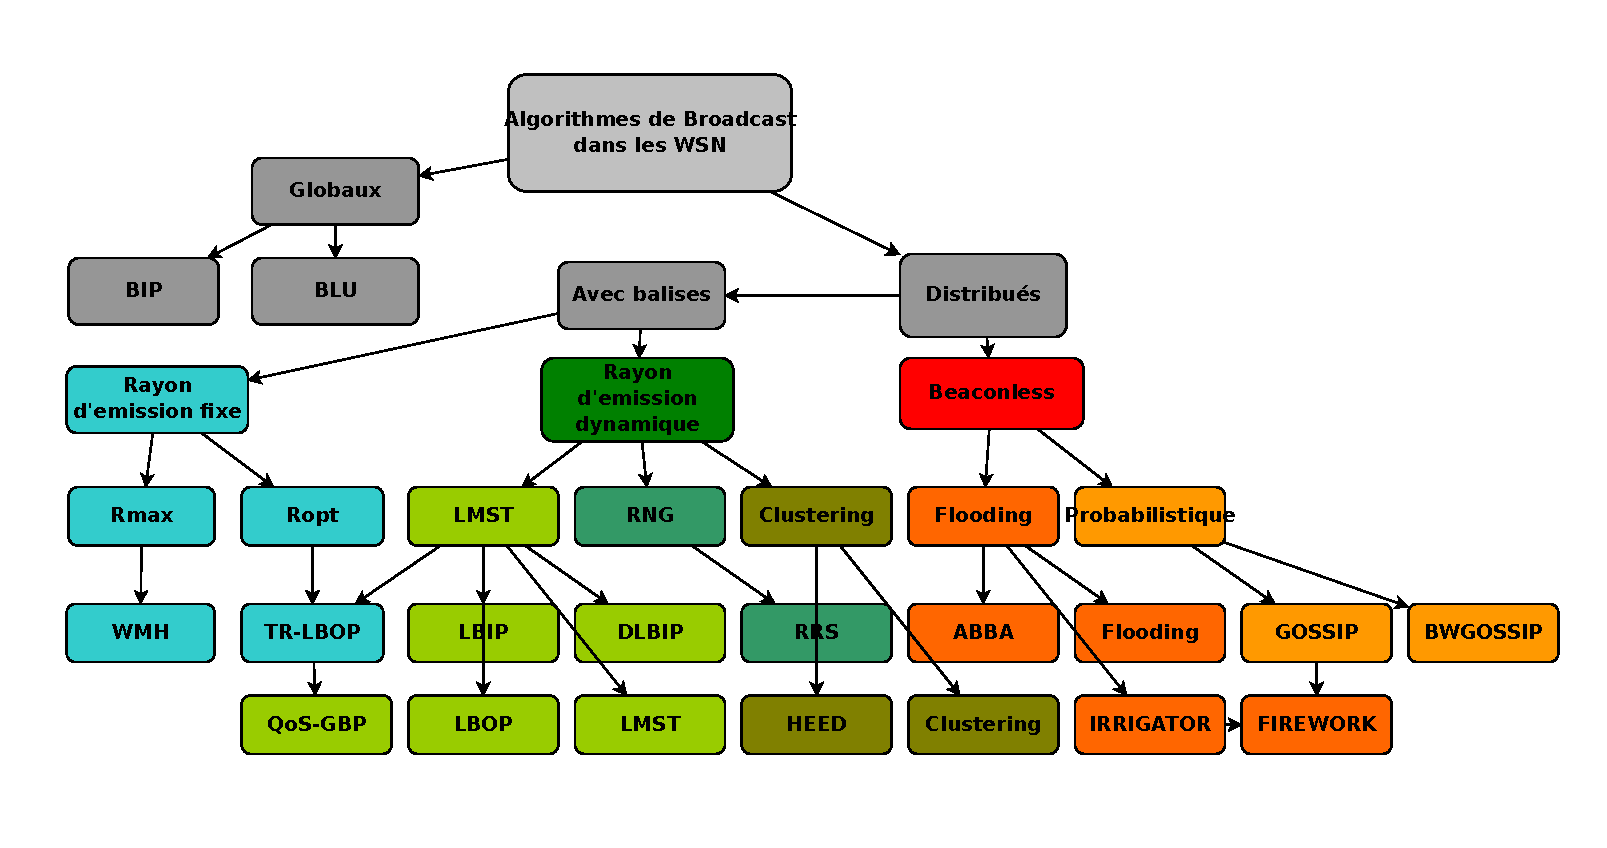
\includegraphics[scale=0.8]{Etat_de_l'art/source/classification}
\caption{ Graphe de synthèse}
\end{figure} 

% TODO : ajouter tableau récapitulatif avec chaque algo sur les lignes et chaque type d'algo sur les colonnes + complexité si possible


